\documentclass{standalone}
\usepackage{tikz}
\usetikzlibrary{patterns, positioning}
\usepackage[sfdefault]{ClearSans} %% option 'sfdefault' activates Clear Sans as the default text font
\usepackage[T1]{fontenc}

\begin{document}
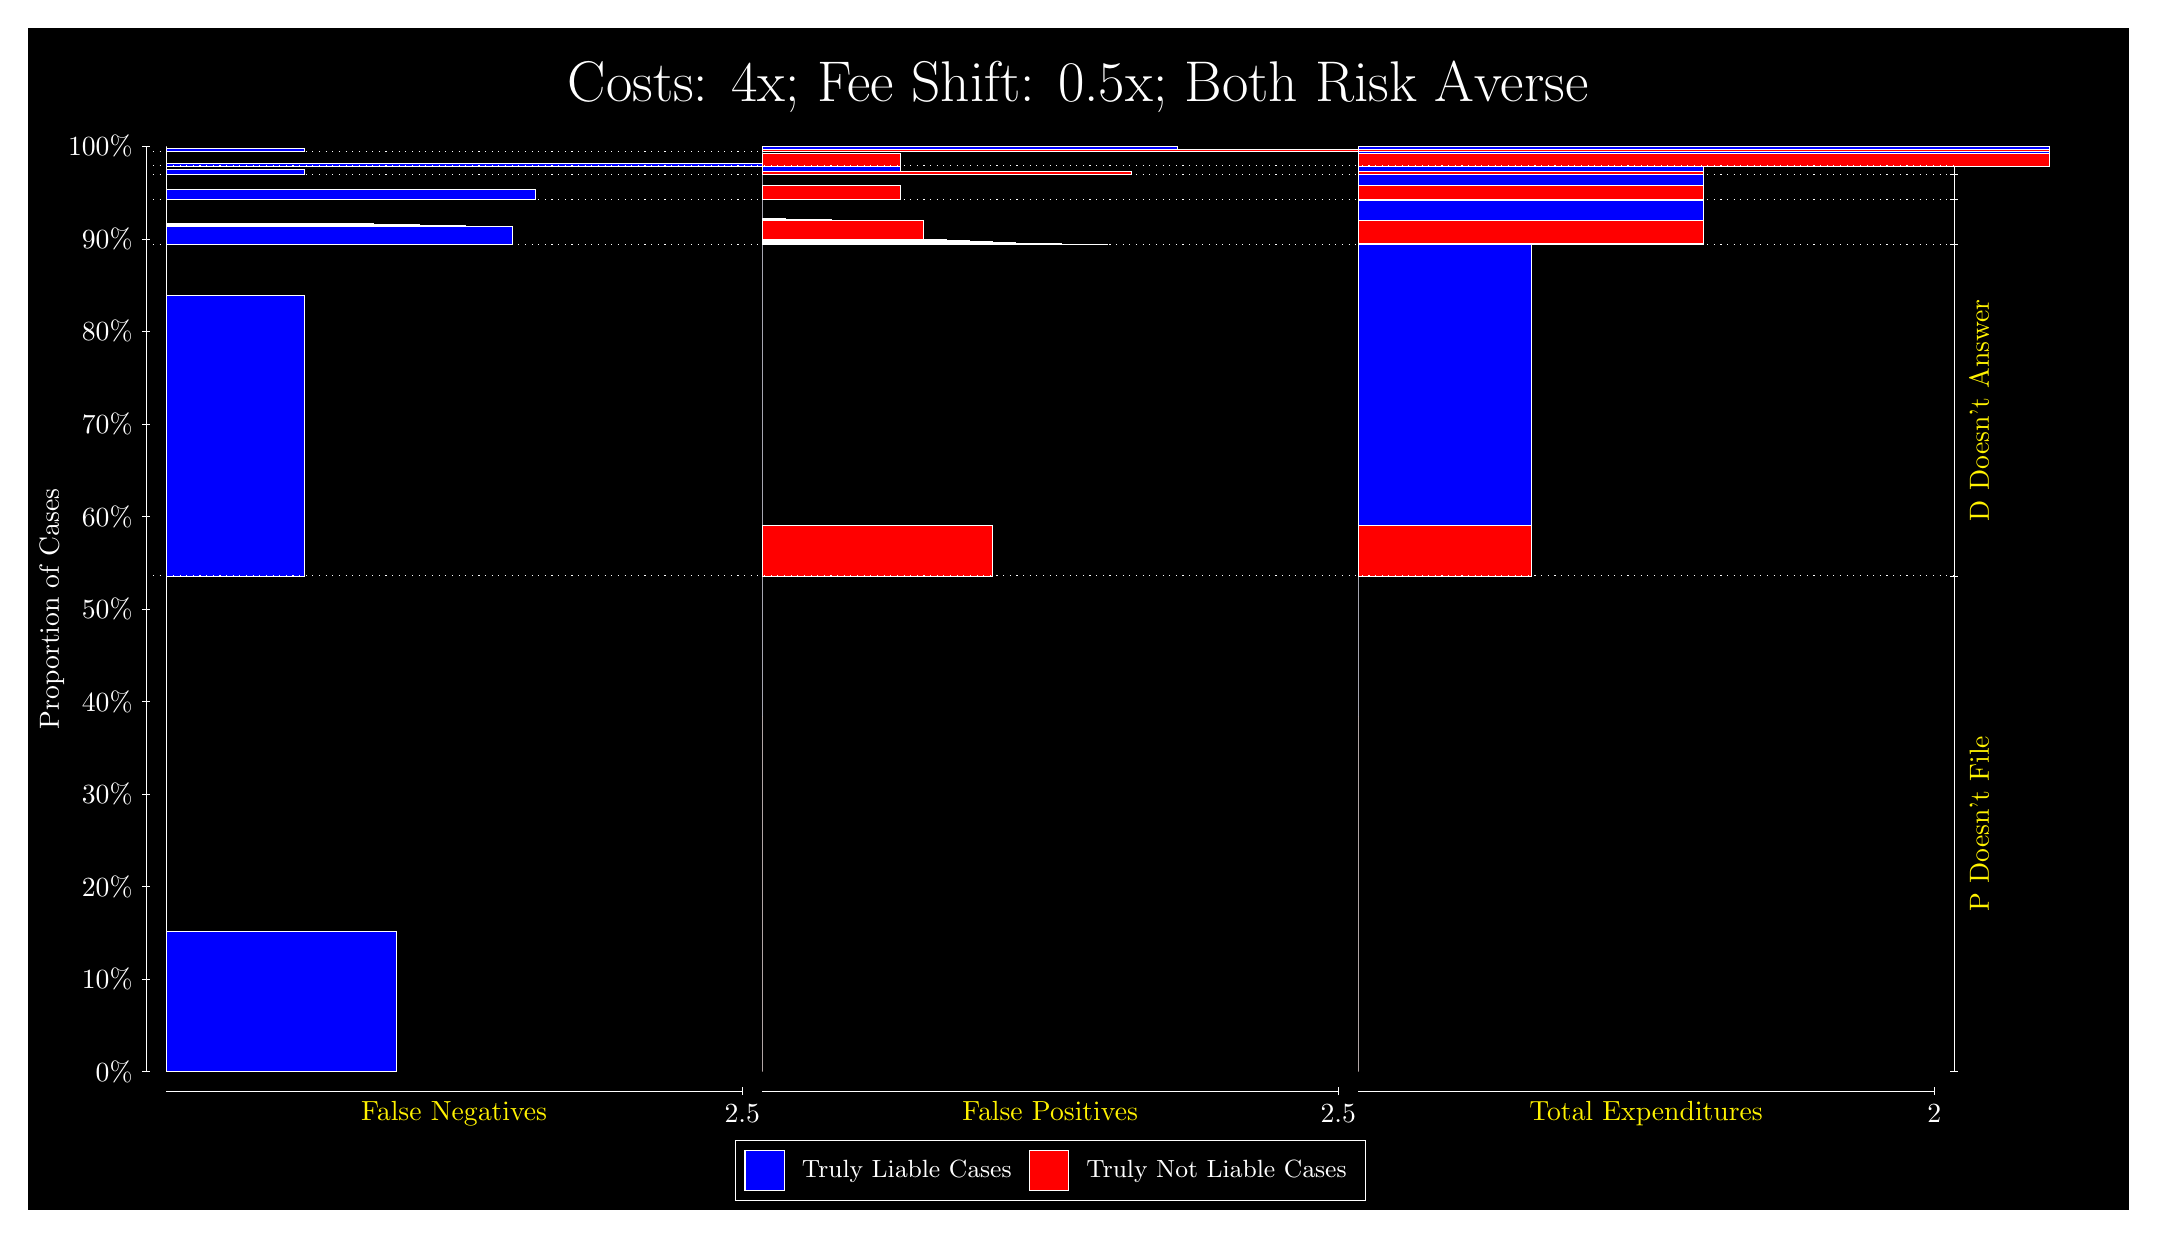
\begin{tikzpicture}
\draw[fill=black] (0,0) rectangle (26.667,15);
\draw[text=white] (0,13.5) rectangle (26.667,15) node[midway] {\huge Costs: 4x; Fee Shift: 0.5x; Both Risk Averse};
\draw[white, very thin] (1.5,1.75) -- (1.5,13.5);
\node[rotate=90, text=white, anchor=center] at (0.3, 7.625) {Proportion of Cases};
\draw[white, very thin] (1.45,1.75) -- (1.55,1.75);
\node[text=white, anchor=east] at (1.45, 1.75) {0\%};
\draw[white, very thin] (1.45,2.925) -- (1.55,2.925);
\node[text=white, anchor=east] at (1.45, 2.925) {10\%};
\draw[white, very thin] (1.45,4.1) -- (1.55,4.1);
\node[text=white, anchor=east] at (1.45, 4.1) {20\%};
\draw[white, very thin] (1.45,5.275) -- (1.55,5.275);
\node[text=white, anchor=east] at (1.45, 5.275) {30\%};
\draw[white, very thin] (1.45,6.45) -- (1.55,6.45);
\node[text=white, anchor=east] at (1.45, 6.45) {40\%};
\draw[white, very thin] (1.45,7.625) -- (1.55,7.625);
\node[text=white, anchor=east] at (1.45, 7.625) {50\%};
\draw[white, very thin] (1.45,8.8) -- (1.55,8.8);
\node[text=white, anchor=east] at (1.45, 8.8) {60\%};
\draw[white, very thin] (1.45,9.975) -- (1.55,9.975);
\node[text=white, anchor=east] at (1.45, 9.975) {70\%};
\draw[white, very thin] (1.45,11.15) -- (1.55,11.15);
\node[text=white, anchor=east] at (1.45, 11.15) {80\%};
\draw[white, very thin] (1.45,12.325) -- (1.55,12.325);
\node[text=white, anchor=east] at (1.45, 12.325) {90\%};
\draw[white, very thin] (1.45,13.5) -- (1.55,13.5);
\node[text=white, anchor=east] at (1.45, 13.5) {100\%};

\draw[white, very thin] (24.457,1.75) -- (24.457,13.5);
\draw[white, very thin] (24.407,1.75) -- (24.507,1.75);
\node[anchor=west] at (24.407, 1.75) {};
\draw[white, very thin] (24.407,8.0443) -- (24.507,8.0443);
\node[anchor=west] at (24.407, 8.0443) {};
\draw[white, very thin] (24.407,12.254) -- (24.507,12.254);
\node[anchor=west] at (24.407, 12.254) {};
\draw[white, very thin] (24.407,12.829) -- (24.507,12.829);
\node[anchor=west] at (24.407, 12.829) {};
\draw[white, very thin] (24.407,13.141) -- (24.507,13.141);
\node[anchor=west] at (24.407, 13.141) {};
\draw[white, very thin] (24.407,13.252) -- (24.507,13.252);
\node[anchor=west] at (24.407, 13.252) {};
\draw[white, very thin] (24.407,13.436) -- (24.507,13.436);
\node[anchor=west] at (24.407, 13.436) {};
\draw[white, very thin] (24.407,13.5) -- (24.507,13.5);
\node[anchor=west] at (24.407, 13.5) {};

\draw[white, very thin, fill=blue] (1.75,1.75) rectangle (4.6775,3.5301);
\draw[white, very thin, fill=red] (1.75,3.5301) rectangle (1.75,8.0443);
\draw[white, very thin, fill=blue] (1.75,8.0443) rectangle (3.5065,11.607);
\draw[white, very thin, fill=red] (1.75,11.607) rectangle (1.75,12.254);
\draw[white, very thin, fill=blue] (1.75,12.254) rectangle (6.1413,12.48);
\draw[white, very thin, fill=blue] (1.75,12.48) rectangle (5.8486,12.489);
\draw[white, very thin, fill=blue] (1.75,12.489) rectangle (5.5558,12.496);
\draw[white, very thin, fill=blue] (1.75,12.496) rectangle (5.2631,12.503);
\draw[white, very thin, fill=blue] (1.75,12.503) rectangle (4.9703,12.512);
\draw[white, very thin, fill=blue] (1.75,12.512) rectangle (4.6775,12.515);
\draw[white, very thin, fill=blue] (1.75,12.515) rectangle (4.3848,12.519);
\draw[white, very thin, fill=blue] (1.75,12.519) rectangle (4.092,12.522);
\draw[white, very thin, fill=blue] (1.75,12.522) rectangle (3.7993,12.523);
\draw[white, very thin, fill=red] (1.75,12.523) rectangle (1.75,12.829);
\draw[white, very thin, fill=blue] (1.75,12.829) rectangle (6.4341,12.958);
\draw[white, very thin, fill=red] (1.75,12.958) rectangle (1.75,13.141);
\draw[white, very thin, fill=blue] (1.75,13.141) rectangle (3.5065,13.21);
\draw[white, very thin, fill=red] (1.75,13.21) rectangle (1.75,13.252);
\draw[white, very thin, fill=blue] (1.75,13.252) rectangle (9.9471,13.28);
\draw[white, very thin, fill=red] (1.75,13.28) rectangle (1.75,13.436);
\draw[white, very thin, fill=blue] (1.75,13.436) rectangle (3.5065,13.473);
\draw[white, very thin, fill=red] (1.75,13.473) rectangle (1.75,13.5);
\draw[white, very thin, fill=red] (9.3189,1.75) rectangle (9.3189,6.2641);
\draw[white, very thin, fill=blue] (9.3189,6.2641) rectangle (9.3189,8.0443);
\draw[white, very thin, fill=red] (9.3189,8.0443) rectangle (12.246,8.6914);
\draw[white, very thin, fill=blue] (9.3189,8.6914) rectangle (9.3189,12.254);
\draw[white, very thin, fill=red] (9.3189,12.254) rectangle (13.71,12.256);
\draw[white, very thin, fill=red] (9.3189,12.256) rectangle (13.417,12.259);
\draw[white, very thin, fill=red] (9.3189,12.259) rectangle (13.125,12.264);
\draw[white, very thin, fill=red] (9.3189,12.264) rectangle (12.832,12.269);
\draw[white, very thin, fill=red] (9.3189,12.269) rectangle (12.539,12.281);
\draw[white, very thin, fill=red] (9.3189,12.281) rectangle (12.246,12.289);
\draw[white, very thin, fill=red] (9.3189,12.289) rectangle (11.954,12.303);
\draw[white, very thin, fill=red] (9.3189,12.303) rectangle (11.661,12.318);
\draw[white, very thin, fill=red] (9.3189,12.318) rectangle (11.368,12.56);
\draw[white, very thin, fill=blue] (9.3189,12.56) rectangle (10.783,12.561);
\draw[white, very thin, fill=blue] (9.3189,12.561) rectangle (10.49,12.564);
\draw[white, very thin, fill=blue] (9.3189,12.564) rectangle (10.197,12.568);
\draw[white, very thin, fill=blue] (9.3189,12.568) rectangle (9.9044,12.571);
\draw[white, very thin, fill=blue] (9.3189,12.571) rectangle (9.6116,12.58);
\draw[white, very thin, fill=blue] (9.3189,12.58) rectangle (9.3189,12.829);
\draw[white, very thin, fill=red] (9.3189,12.829) rectangle (11.075,13.011);
\draw[white, very thin, fill=blue] (9.3189,13.011) rectangle (9.3189,13.141);
\draw[white, very thin, fill=red] (9.3189,13.141) rectangle (14.003,13.183);
\draw[white, very thin, fill=blue] (9.3189,13.183) rectangle (11.075,13.252);
\draw[white, very thin, fill=red] (9.3189,13.252) rectangle (11.075,13.408);
\draw[white, very thin, fill=blue] (9.3189,13.408) rectangle (9.3189,13.436);
\draw[white, very thin, fill=red] (9.3189,13.436) rectangle (17.516,13.463);
\draw[white, very thin, fill=blue] (9.3189,13.463) rectangle (14.588,13.5);
\draw[white, very thin, fill=red] (16.888,1.75) rectangle (16.888,6.2641);
\draw[white, very thin, fill=blue] (16.888,6.2641) rectangle (16.888,8.0443);
\draw[white, very thin, fill=red] (16.888,8.0443) rectangle (19.083,8.6914);
\draw[white, very thin, fill=blue] (16.888,8.6914) rectangle (19.083,12.254);
\draw[white, very thin, fill=red] (16.888,12.254) rectangle (21.279,12.266);
\draw[white, very thin, fill=blue] (16.888,12.266) rectangle (21.279,12.274);
\draw[white, very thin, fill=red] (16.888,12.274) rectangle (21.279,12.561);
\draw[white, very thin, fill=blue] (16.888,12.561) rectangle (21.279,12.814);
\draw[white, very thin, fill=red] (16.888,12.814) rectangle (21.279,12.822);
\draw[white, very thin, fill=blue] (16.888,12.822) rectangle (21.279,12.829);
\draw[white, very thin, fill=red] (16.888,12.829) rectangle (21.279,13.011);
\draw[white, very thin, fill=blue] (16.888,13.011) rectangle (21.279,13.141);
\draw[white, very thin, fill=red] (16.888,13.141) rectangle (21.279,13.183);
\draw[white, very thin, fill=blue] (16.888,13.183) rectangle (21.279,13.252);
\draw[white, very thin, fill=red] (16.888,13.252) rectangle (25.67,13.408);
\draw[white, very thin, fill=blue] (16.888,13.408) rectangle (25.67,13.436);
\draw[white, very thin, fill=red] (16.888,13.436) rectangle (25.67,13.463);
\draw[white, very thin, fill=blue] (16.888,13.463) rectangle (25.67,13.5);
\draw[white, dotted] (1.5,8.0443) -- (24.457,8.0443);
\draw[white, dotted] (1.5,12.254) -- (24.457,12.254);
\draw[white, dotted] (1.5,12.829) -- (24.457,12.829);
\draw[white, dotted] (1.5,13.141) -- (24.457,13.141);
\draw[white, dotted] (1.5,13.252) -- (24.457,13.252);
\draw[white, dotted] (1.5,13.436) -- (24.457,13.436);
\draw[white, very thin] (1.75,1.5) -- (9.0689,1.5);
\node[text=yellow, anchor=north] at (5.4094, 1.5) {False Negatives};
\draw[white, very thin] (9.0689,1.45) -- (9.0689,1.55);
\node[text=white, anchor=north] at (9.0689, 1.45) {2.5};

\draw[white, very thin] (9.3189,1.5) -- (16.638,1.5);
\node[text=yellow, anchor=north] at (12.978, 1.5) {False Positives};
\draw[white, very thin] (16.638,1.45) -- (16.638,1.55);
\node[text=white, anchor=north] at (16.638, 1.45) {2.5};

\draw[white, very thin] (16.888,1.5) -- (24.207,1.5);
\node[text=yellow, anchor=north] at (20.547, 1.5) {Total Expenditures};
\draw[white, very thin] (24.207,1.45) -- (24.207,1.55);
\node[text=white, anchor=north] at (24.207, 1.45) {2};

\node[text=yellow, centered, rotate=90] at (24.777, 4.8971) {P Doesn't File};
\node[text=yellow, centered, rotate=90] at (24.777, 10.149) {D Doesn't Answer};






\draw (12.978300999999998,1.5) node[draw=none] (baseCoordinate) {};
\begin{scope}[align=center]
        \matrix[scale=0.5, draw=white, below=0.5cm of baseCoordinate, nodes={draw}, column sep=0.1cm]{
            \node[rectangle, draw, minimum width=0.5cm, minimum height=0.5cm, fill=blue] {}; &
            \node[draw=none, font=\small, text=white] (B) {Truly Liable Cases}; &
            \node[rectangle, draw, minimum width=0.5cm, minimum height=0.5cm, fill=red] {}; &
            \node[draw=none, font=\small, text=white] (B) {Truly Not Liable Cases}; \\
            };
\end{scope}

\end{tikzpicture}
\end{document}